%\newacronym{relu}{ReLU}{Rectified Linear Unit}

\section{Machine Learning}\label{sec:theory-machine-learning}
Understanding the basics of machine learning is important to determine the appropriate dimensionality reduction methods to compare for the project. This section will describe the basics of machine learning by describing a simplified model of a machine learning model pipeline.


\subsection{Machine learning pipeline}\label{subsec:machine-learning-pipeline}
\autoref{fig:basic-machine-learning-pipeline} shows the simplified and generalized steps in the pipeline of a machine-learning model. The arrows represent how machine learning models continuously learn. The model is trained on the training set and then evaluated on the validation set. The model then updates with the new information, and the process repeats. This loop is called the training loop. The training loop repeats until the model converges or until the model is no longer improving. The model gets evaluated on the test set, and the evaluation gets used to determine the model's performance. The reason for having a pipeline for a machine learning model states as follows:

\blockcquote{machine-learning-pipeline-architecture}{A machine learning pipeline (or system) is a technical infrastructure used to manage and automate ML processes in the organization. The pipeline logic and the number of tools it consists of vary depending on the ML needs. But, in any case, the pipeline would provide data engineers with means of managing data for training, orchestrating models, and managing them on production.}

For this simplified example, the machine learning pipeline shown in this report has four main steps: data collection, feature engineering, model training, and model Evaluation. This model is not entirely identical to the model shown in~\cite{machine-learning-pipeline-architecture}, as this is a simplified model with slight modifications to fit this project's scope. The four steps will get described in the following subsections.


% \begin{figure}[htb!]
%     \centering
%     \begin{tikzpicture}
%         \node (b) [state] {feature engineering};
%         \node (c) [state, shift={($(b.east)+(2cm,0)$)}] {model};
%         \node (a) [state, shift={($(b.west)+(-2cm,0)$)}] {data};
%         \node (d) [state, shift={($(c.east)+(2cm,0)$)}] {evaluation};
%         \node (e) [state, shift={($(b.south)+(0,-2cm)$)}] {parameters};

%         \draw[arrow, ->] (a) -- node[above,scale=.70,align=center,] {} (b);
%         \draw[arrow, ->] (b) -- node[above,scale=.70,align=center,] {} (c);
%         \draw[arrow, ->] (c) -- node[above,scale=.70,align=center,] {} (d);
%         \draw[arrow, ->] (e) -- node[above,scale=.70,align=center,] {} (c);

%         \draw[arrow, ->] (d.north) -- ++(0,0.75) -| (b);
%         \draw[arrow, ->] (d.south) -- ++(0,-0.75) -| (c);
%     \end{tikzpicture}
%     \caption{Simplified machine learning pipeline}
%     \label{fig:machine-learning-pipeline}
% \end{figure}

\subsubsection{Data collection}\label{subsubsec:machine-learning-pipeline-data-collection}
The \texttt{data} box in \autoref{fig:basic-machine-learning-pipeline} represents the collection of data to be used in training the machine learning model~\cite{machine-learning-pipeline-architecture}. There are many different types of data, but some of the most commonly used, as stated by \cite{the-importance-of-machine-learning-data}, are Numerical Data, Categorical Data, Time Series Data, and Text Data. Often the data is in some type or format which is not directly usable by the machine learning model. For this, the \texttt{feature engineering} step is used.

\subsubsection{Feature engineering}\label{subsubsec:machine-learning-pipeline-feature-engineering}
\texttt{Feature engineering} represents the step where the data gets transformed through dimensionality reduction. In~\cite{machine-learning-pipeline-architecture}, \texttt{Data preparation} and \texttt{feature engineering} are both in a step called \texttt{prepare data}, for this model, \texttt{feature engineering} covers those steps. \texttt{feature engineering} is also the step where data is preprocessed~\cite{machine-learning-pipeline-architecture}. Preprocessing is done to ensure quality data~\cite{data-preparation-for-data-mining}, and feature engineering is done, among other reasons, to improve the quality of the results, and to improve the performance of the machine learning model, by reducing the burden on the machine learning algorithms~\cite{dimensionality-reduction-reddy}.

\subsubsection{Model}\label{subsubsec:machine-learning-pipeline-model-training}
\texttt{model} is where the process of training the model with the data takes place. Model training splits the data into a training set and a validation set. An example of model training gets seen in further detail in the model shown in~\cite{machine-learning-pipeline-architecture}, at the \texttt{Split data} step. As stated in~\ref{sec:cross-validation}, it is important to split the data in this manner, as it helps to reduce the risk of overfitting.

\subsubsection{Evaluation}\label{subsubsec:machine-learning-pipeline-evaluation}
\texttt{evaluation} represents the step where the model trained on the training set, gets evaluated on the validation set. The evaluation compares the model's predictions with the actual values. The model's predictions get evaluated on the validation set, and this step can repeat multiple times~\cite{machine-learning-pipeline-architecture}. Using accuracy, precision, recall, and F1 score metrics helps provide information regarding the performance of the model~\cite{performance-evaluation}.

\subsubsection{Parameters}\label{subsubsec:machine-learning-pipeline-parameters}
\texttt{Parameters} represents the step where hyperparameters of the machine learning model get set and tuned. The algorithm sets some parameters through training, then there are hyperparameters, which are parameters given to the algorithms to train the model~\cite{what-is-hyperparameter-tuning}. This step is purely for hyperparameters. As mentioned in the previous section \ref{sec:hyperparam}, there are multiple ways to tune hyperparameters. The main reason this tuning is important is that it helps improve the model's performance and reduce the risk of overfitting~\cite{hyperparameter-tuning}.





% \subsection{Data}\label{subsec:data}
% Because the machine learning pipeline starts with the data, the choice of dataset for the project will impact all the following steps in the pipeline.

% Most importantly the data must allow for the evaluation of the dimensionality reduction methods. Therefore, the dataset should be large enough dimensionally to perform meaningful dimensionality reduction. Furthermore, a well researched dataset is preferred, as it is more likely to be well suited for the evaluation of dimensionality reduction methods.

% Based on the above requirements the \gls{mnist}~\cite{lecun-mnist-database} dataset is chosen. It is a dataset of images of 28x28 grayscale images of handwritten digits, making it well suited for the evaluation of dimensionality reduction methods, as the images are large enough to perform meaningful dimensionality reduction. Furthermore, the dataset is well researched, and has been used in many papers~\cite{lecun-mnist-database}.

% In fact \gls{mnist} is so well researched that it may be considered overused~\cite{fashion-mnist}. If time permits, two similar datasets may be used in the project. The first is the \gls{fashion-mnist}~\cite{fashion-mnist} dataset, which is a variant of \gls{mnist} with images of clothing instead of handwritten digits. The second is the \gls{cifar}~\cite{krizhevsky-cifar} dataset, which consists of 50,000 training images and 10,000 test images of 32x32 color images of 10 different classes of objects.


% \subsection{Feature engineering}\label{subsec:feature-engineering}
% The theory deciding the choice of dimensionality reduction methods is described in Chapter~\ref{cha:theory}.

% \todo[inline]{Some notes: normal distribution is relevant for LDA in particular apparently \url{https://www.rikvoorhaar.com/normal-data/}. FA is unlikely to be practical. PCA is the most common method}

% %Moved into classification


% \subsubsection{Convolutional Neural Networks}\label{subsubsec:convolutional-neural-networks}
% We assume that the reader is familiar with \gls{nn}s. The \gls{cnn}s are a specialized form of \gls{nn} that are mostly used for pattern recognition in images~\cite{introduction-to-cnn}. The reason we chose to work with \gls{cnn} is because, while normal \gls{nn}s are able to solve the classification problem regarding \gls{mnist}, they might not be as powerful as \gls{cnn}. The robustness of the \gls{cnn} can be shown in the sources~\cite{lecun-mnist-database, mnist-classification-benchmark}, where \gls{cnn}s are depicted as being 'state-of-the-art' machine learning models based on the minimum error rate that they achieve.


% In our project it might not make a major difference, but using a \gls{cnn} can be better suited for image classifcation, as presented. Furthermore, according to Keiron et al.\ ~\cite{introduction-to-cnn}, \gls{nn}s are more prone to overfitting due to the layers being fully-connected, which increases the number of parameters, thereby increasing the complexity of the model. Another reason is the practicality / scalability of the model, as Keiron highlighted in his report, where he depicted a possible issue with \gls{nn}. The \gls{mnist} consists of $28 \times 28$ \textit{monochrome} pixels, which is relatively simple, compared to the real-world images which can be bigger, and have three colors / channels. We know that \gls{nn}s are fully-connected layers, in essence, neurons are connected to all the neurons in the previous layer, and Figure \ref{fig:nn-example-architecture} can provide a visual aid. When the amount of pixels is large, and colorized, then so should the size of the \gls{nn} be~\cite{introduction-to-cnn}.

% \begin{figure}[htb!]
%     \centering
%     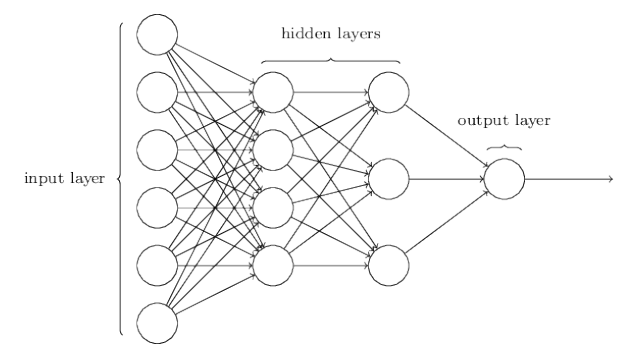
\includegraphics[width=0.65\textwidth]{figures/michael-nielsen-nn-architecture.png}
%     \caption{An example of a neural network architecture~\cite{michael-nielsen-nn}}
%     \label{fig:nn-example-architecture}
% \end{figure}

% The difference between \gls{nn} and \gls{cnn} is the among others the architectural blueprint. In \gls{cnn} neurons also have another property: the neurons are arranged in three dimensions: \textcquote{introduction-to-cnn}{the spatial dimensionality of the input(\textbf{height} and the \textbf{width}), and the \textbf{depth}}. The spatial dimensionality is the pixels, and the depth is one, since \gls{mnist} is monochrome.


% %Ugly figure and not 100% visual, but it is simple
% \begin{figure}[htb!]
%     \centering
%     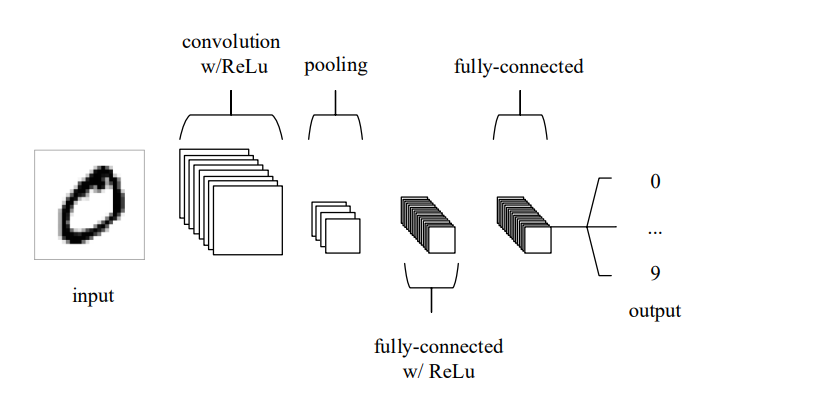
\includegraphics[width=0.8\textwidth]{figures/cnn-simple-architecture.png}
%     \caption{An example of a convolutional neural network architecture~\cite{introduction-to-cnn}}
%     \label{fig:simple-cnn-architecture}
% \end{figure}
% %Blog-like structure where CNN is depicted

% \gls{cnn}'s architecture constitutes three different types of layers: convolutional layers, pooling layers, and fully-connected layers. The architecture of a \gls{cnn} can be shown in Figure \ref{fig:simple-cnn-architecture}. The convolutional layers \textcquote{introduction-to-cnn}{will determine the output of neurons of which are connected to local regions of the input}, which is also called a convolution. The pooling layers reduce the number of parameters in the previous layers. The fully-connected layers act as normal \gls{nn} layers~\cite{introduction-to-cnn}.


% A convolution, as described, acts as a filter which maps the input to an output matrix $conv$ of size $n \times n$. The mapping is done by the elementwise-multiplication of the input matrix with the $conv$ matrix. The operation can be seen in Figure \ref{fig:convolution}. The manner in which such mapping is achieved is by sliding over the input matrix, from left to right, top to bottom, with a $n \times n$ matrix one pixel at a time. For each convolution operation \gls{relu} is applied to the operation, where \gls{relu} is a function which takes the maximum value between 0 and the input~\cite{google-cnn}.

% \begin{figure}[htb!]
%     \centering
%     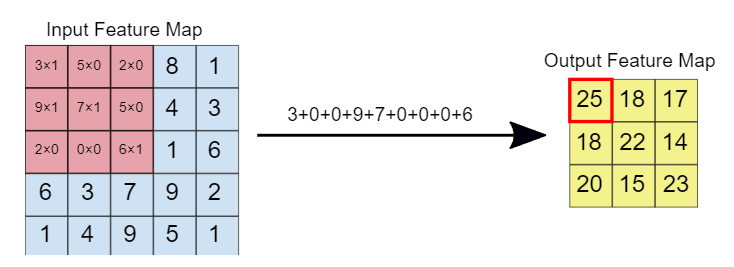
\includegraphics[width=0.7\textwidth]{figures/google-cnn-convolution-example.png}
%     \caption{An example of a convolution operation~\cite{google-cnn}}
%     \label{fig:convolution}
% \end{figure}

% In the pooling layer behaves like a convolution, but this time it filters the $conv$ matrix with a $pool$ matrix of size $n \times n$. One method which has been presented~\cite{google-cnn} is the use of max pooling; in the convolutional layer the elementwise multiplication is applied, whereas in max pooling the element with the highest number in the respective matrix is chosen~\cite{google-cnn}. Figure \ref{fig:maxpooling} is provided to show how it works. The pooling layer can be seen as a dimensionality reduction method, because it reduces the data while preserving the original features.

% \begin{figure}[htb!]
%     \centering
%     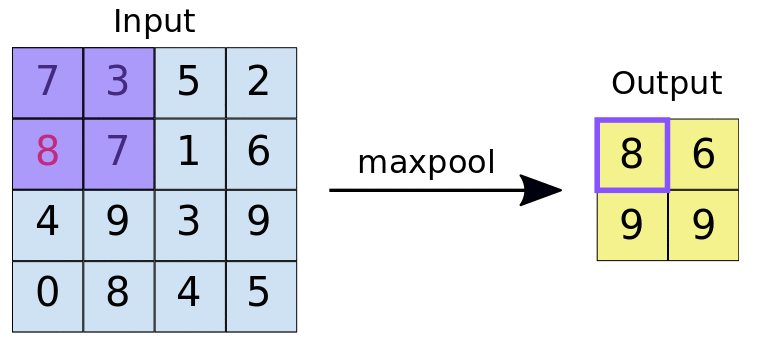
\includegraphics[width=0.5\textwidth]{figures/google-cnn-maxpooling-example.png}
%     \caption{An example of a max pooling operation~\cite{google-cnn}}
%     \label{fig:maxpooling}
% \end{figure}

% The last layer is the fully-connected layer, which is connected to all the neurons from the pooling layer. According to Keiron ~\cite{introduction-to-cnn}, the activation function \gls{relu} might be suited to be used in this layer too~\cite{lecun-mnist-database}.

% \subsection{Model training}\label{subsec:model-training}
% The theory deciding the cross validation methods is described in Chapter~\ref{cha:theory}.



% @book{michael-nielsen-nn,
%   title={Neural networks and deep learning},
%   author={Nielsen, Michael A},
%   volume={25},
%   year={2015},
%   publisher={Determination press San Francisco, CA, USA}
% }

% @misc{faster-svm,
%   doi = {10.48550/ARXIV.1808.06394},
%   url = {https://arxiv.org/abs/1808.06394},
%   author = {Schlag, Sebastian and Schmitt, Matthias and Schulz, Christian},
%   title = {Faster Support Vector Machines},
%   publisher = {arXiv},
%   year = {2018},
%   copyright = {arXiv.org perpetual, non-exclusive license}
% }

% @misc{introduction-to-cnn,
%   doi = {10.48550/ARXIV.1511.08458},
%   url = {https://arxiv.org/abs/1511.08458},
%   author = {O'Shea, Keiron and Nash, Ryan},
%   title = {An Introduction to Convolutional Neural Networks},
%   publisher = {arXiv},
%   year = {2015},
%   copyright = {arXiv.org perpetual, non-exclusive license}
% }

% @misc{mnist-classification-benchmark,
%     url = {https://paperswithcode.com/sota/image-classification-on-mnist},
%     title = {Image Classifcation onf MNIST},
%     year = {2022}
% }

% @misc{google-cnn,
%     organization = {Google},
%     url = {https://developers.google.com/machine-learning/practica/image-classification/convolutional-neural-networks},
%     title = {ML Practicum: Image Classification},
%     year = {2022}
% }

% @misc{machine-learning-pipeline-architecture,
% author       = {Altexsoft},
% url          = {https://www.altexsoft.com/blog/machine-learning-pipeline/},
% title        = {Machine Learning Pipeline: Architecture of ML Platform in Production},
% urldate      = {2022-11-23}
% }

% @misc{the-importance-of-machine-learning-data,
% author       = {DataRobot},
% url          = {https://www.datarobot.com/blog/the-importance-of-machine-learning-data/},
% title        = {The importance of machine learning data},
% urldate      = {2022-11-23}
% }

% @INPROCEEDINGS{performance-evaluation,
%   author={Behera, Bichitrananda and Kumaravelan, G. and Kumar B., Prem},
%   booktitle={2019 11th International Conference on Advanced Computing (ICoAC)}, 
%   title={Performance Evaluation of Deep Learning Algorithms in Biomedical Document Classification}, 
%   year={2019},
%   doi={10.1109/ICoAC48765.2019.246843}
% }

% @inproceedings{lavesson2006quantifying,
%   title={Quantifying the impact of learning algorithm parameter tuning},
%   author={Lavesson, Niklas and Davidsson, Paul},
%   booktitle={AAAI},
%   year={2006}
% }

